\documentclass{standalone}
\usepackage{tikz}

\begin{document}

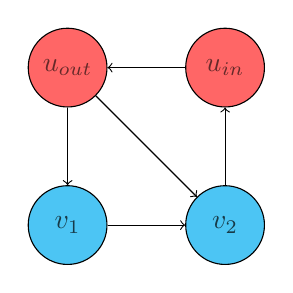
\begin{tikzpicture}
    \node[shape=circle,draw=black,fill=cyan, fill opacity=0.7, minimum size = 1cm] (v1) at (0,0) {$v_1$};
    \node[shape=circle,draw=black,fill=cyan, fill opacity=0.7, minimum size = 1cm] (v2) at (2,0) {$v_2$};
    \node[shape=circle,draw=black,fill=red, fill opacity=0.6, minimum size = 1cm] (v3) at (2,2) {$u_{in}$};
    \node[shape=circle,draw=black,fill=red, fill opacity=0.6, minimum size = 1cm] (v4) at (0,2) {$u_{out}$};
    % Your additional code here
    \path [->] (v1) edge node[left] {} (v2);
    \path [->] (v2) edge node[left] {} (v3);
    \path [->] (v3) edge node[left] {} (v4);
    \path [->] (v4) edge node[left] {} (v1);
    \path [->] (v4) edge node[left] {} (v2);
\end{tikzpicture}

\end{document}